\chapter{Materiais e Métodos}

\section{Metodologia}
O desenvolvimento deste projeto seguiu uma abordagem iterativa e incremental, baseando-se em metodologias ágeis em oposição ao modelo tradicional em cascata (\textit{waterfall}). Enquanto o modelo cascata prevê uma sequência rígida de fases (requisitos, projeto, implementação, testes e manutenção), as metodologias ágeis permitem a adaptação contínua e a entrega frequente de valor~\cite{sommerville2011software}.

Dentre as práticas ágeis, foram utilizados princípios do \textit{Scrum}, como a divisão do trabalho em ciclos curtos e a revisão constante dos requisitos. Essa flexibilidade foi crucial para lidar com a complexidade da ferramenta, permitindo refinamento da solução a cada iteração. Além disso, a arquitetura do sistema foi guiada pelos princípios do \textit{Domain-Driven Design} (DDD)~\cite{evans2004domain}, garantindo que a lógica de negócio (o domínio da regressão simbólica) permanecesse isolada das complexidades de infraestrutura, como banco de dados e brokers de mensagens, o que permite a substituição de implementações específicas por outras desde que a interface definida pela aplicação seja respeitada.

\section{Ambiente de Desenvolvimento e Ferramentas}
O projeto foi desenvolvido utilizando o Windows Subsystem for Linux (WSL), uma ferramenta que permite a criação de máquinas virtuais Linux dentro de um computador Windows, e Docker, uma ferramenta que permite a conteinerização de aplicações.

O Docker foi utilizado para facilitar o gerenciamento do ambiente de desenvolvimento back-end, permitindo a criação de dois serviços essenciais para a aplicação: Postgres (Banco de Dados Relacional) e RabbitMQ (Broker de Mensagens). O uso dessa ferramenta permite a replicabilidade do ambiente de desenvolvimento em qualquer máquina, facilitando o processo de criação e execução do código.

\subsection{Desenvolvimento Front-end}
A construção das telas da plataforma e suas funcionalidades foi feita através do \textit{framework} React (desenvolvido e mantido pela Meta) que utiliza a linguagem imperativa \textit{JavaScript}. Além disso, as bibliotecas \textit{Tanstack React Query} e \textit{Zustand} foram utilizadas, respectivamente, para gerenciamento de estado assíncrono, ou seja, informações vindas diretamente do back-end da aplicação, e para gerenciamento do estado interno da aplicação front-end.

Demais ferramentas utilizadas e suas versões específicas podem ser encontradas abaixo:
\begin{lstlisting}[language=json, caption=Bibliotecas utilizadas no front-end e suas versões]
"dependencies": {
    "@hookform/resolvers": "^5.2.2",
    "@monaco-editor/react": "^4.8.0-rc.3",
    "@react-router/node": "^7.9.2",
    "@react-router/serve": "^7.9.2",
    "@tanstack/react-query": "^5.90.21",
    "@tanstack/react-query-devtools": "^5.91.3",
    "@tanstack/react-table": "^8.21.3",
    "clsx": "^2.1.1",
    "framer-motion": "^12.35.2",
    "isbot": "^5.1.31",
    "lucide-react": "^0.577.0",
    "papaparse": "^5.5.3",
    "react": "^19.1.1",
    "react-dom": "^19.1.1",
    "react-dropzone": "^14.3.8",
    "react-hook-form": "^7.69.0",
    "react-intersection-observer": "^10.0.3",
    "react-katex": "^3.1.0",
    "react-markdown": "^10.1.0",
    "react-router": "^7.9.2",
    "rehype-highlight": "^7.0.2",
    "remark-gfm": "^4.0.1",
    "tailwind-merge": "^3.4.0",
    "uuid": "^13.0.0",
    "zod": "^4.3.6",
    "zustand": "^5.0.11"
},
"devDependencies": {
    "@react-router/dev": "^7.9.2",
    "@tailwindcss/typography": "^0.5.19",
    "@tailwindcss/vite": "^4.1.13",
    "@types/node": "^22",
    "@types/papaparse": "^5.5.2",
    "@types/react": "^19.1.13",
    "@types/react-dom": "^19.1.9",
    "@types/react-katex": "^3.0.4",
    "tailwindcss": "^4.1.13",
    "typescript": "^5.9.2",
    "vite": "^7.1.7",
    "vite-tsconfig-paths": "^5.1.4"
}
\end{lstlisting}

Para permitir o treinamento de modelos de regressão de forma assíncrona, evitando o bloqueio do servidor HTTP, o sistema utiliza \textit{workers} independentes em Python que se comunicam com a API principal através do \textit{RabbitMQ}, integrado via biblioteca \textit{aio\_pika}. Por fim, as operações de regressão simbólica foram feitas utilizando as bibliotecas \textit{eggp} para o treinamento, e \textit{rEGGression} para manipulação dos modelos. O \textit{PostgreSQL} foi o banco de dados escolhido devido à natureza fortemente estruturada e relacional das entidades do sistema.

\subsection{Estrutura do Projeto}
A organização do código-fonte segue uma estrutura modular para facilitar a manutenção e o desacoplamento entre os componentes. Abaixo é apresentada a árvore de diretórios principal:

\dirtree{%
.1 spectrum/.
.2 docker/\DTcomment{Configurações de containers (Postgres, RabbitMQ)}.
.2 packages/.
.3 backend/\DTcomment{API FastAPI e lógica de aplicação}.
.3 core/\DTcomment{Domínio puro, entidades e interfaces (ports)}.
.3 db\_core/\DTcomment{Implementação de repositórios e SQLAlchemy}.
.3 frontend/\DTcomment{Interface React e gerenciamento de estado}.
.3 inference\_query\_language/\DTcomment{Parser e executor da IQL}.
.3 workers/\DTcomment{Processamento especializado assíncrono}.
.2 paper/\DTcomment{Código-fonte LaTeX da monografia}.
.2 scripts/\DTcomment{Utilitários de desenvolvimento e automação}.
}

Cada pacote possui uma responsabilidade bem definida: o \textit{core} isola a lógica de negócio da aplicação, definindo as entidades principais do projeto e as interfaces necessárias para manipulação dessas entidades; o \textit{db\_core} lida exclusivamente com a persistência, definindo as tabelas do banco de dados, bem como as interfaces responsáveis pela manipulação dos dados por meio de operações intermediadas pelo banco de dados; o \textit{backend} orquestra as requisições HTTP e a comunicação com os \textit{workers} via \textit{RabbitMQ}; o \textit{frontend} provê a camada de interação com o usuário final; e o \textit{inference\_query\_language} isola a lógica da linguagem de domínio IQL, utilizada para interagir com os modelos de regressão via sintaxe similar ao SQL.

Demais ferramentas utilizadas e suas versões específicas podem ser encontradas abaixo:
\begin{lstlisting}[language=Toml, caption={Ferramentas utilizadas no back-end e suas versões}]
// Servidor
dependencies = [
    "aio-pika>=9.5.8",
    "aiofiles>=25.1.0",
    "alembic>=1.18.3",
    "asyncpg>=0.31.0",
    "core",
    "db-core",
    "dotenv>=0.9.9",
    "eggp>=1.0.16",
    "fastapi[standard]>=0.128.0",
    "inference-query-language",
    "pandas>=3.0.0",
    "pika>=1.3.2",
    "pydantic[email]>=2.12.5",
    "pydantic-settings>=2.12.0",
    "python-json-logger>=4.0.0",
    "reggression>=1.0.10",
    "sqlalchemy>=2.0.46",
    "uvicorn[standard]",
    "argon2-cffi>=25.1.0",
    "jose>=1.0.0",
    "python-jose[cryptography]>=3.5.0",
]

[tool.uv]
dev-dependencies = [
    "pytest",
    "pytest-asyncio",
    "httpx",
    "ruff",
    "mypy",
    "pre-commit",
]

// Pacote Core
dependencies = [
    "inference-query-language",
    "pydantic>=2.12.5",
    "pydantic-settings>=2.12.0",
    "reggression>=1.0.10",
]

// Pacote DB Core
dependencies = [
    "core",
]

// Pacote IQL
dependencies = [
    "pandas>=3.0.0",
    "pydantic>=2.12.5",
]

// Pacote Workers
dependencies = [
    "eggp>=1.0.16",
    "core",
    "db-core",
    "aio-pika>=9.5.8",
]
\end{lstlisting}

\section{Arquitetura}

A arquitetura da plataforma foi projetada sob o modelo cliente-servidor~\cite{sommerville2011software} com o objetivo de oferecer desacoplamento entre a interface gráfica (front-end) utilizada pelo usuário e a lógica de processamento, ou regras de negócio, e persistência de dados (back-end), permitindo a evolução independente de ambos os sistemas.

Nesta seção, é apresentado o fluxo geral de integração dos componentes do sistema, detalhando os padrões de projeto adotados, baseando-se nos princípios do \textit{Domain Driven Design}~\cite{evans2004domain}, uma forma de desenvolvimento de \textit{software} que preza pelo desenvolvimento dentro de domínios específicos, ou seja, dentro de micro-universos que representam as regras de negócio da aplicação. No capítulo seguinte será apresentado os detalhes de implementação da plataforma, bem como suas principais funcionalidades e também pontos de melhoria e exploração futuros.

\subsection{Visão Geral e Fluxo de Dados}
\begin{figure}
  \centering
  \caption{Diagrama de alto nível da arquitetura do projeto.}
  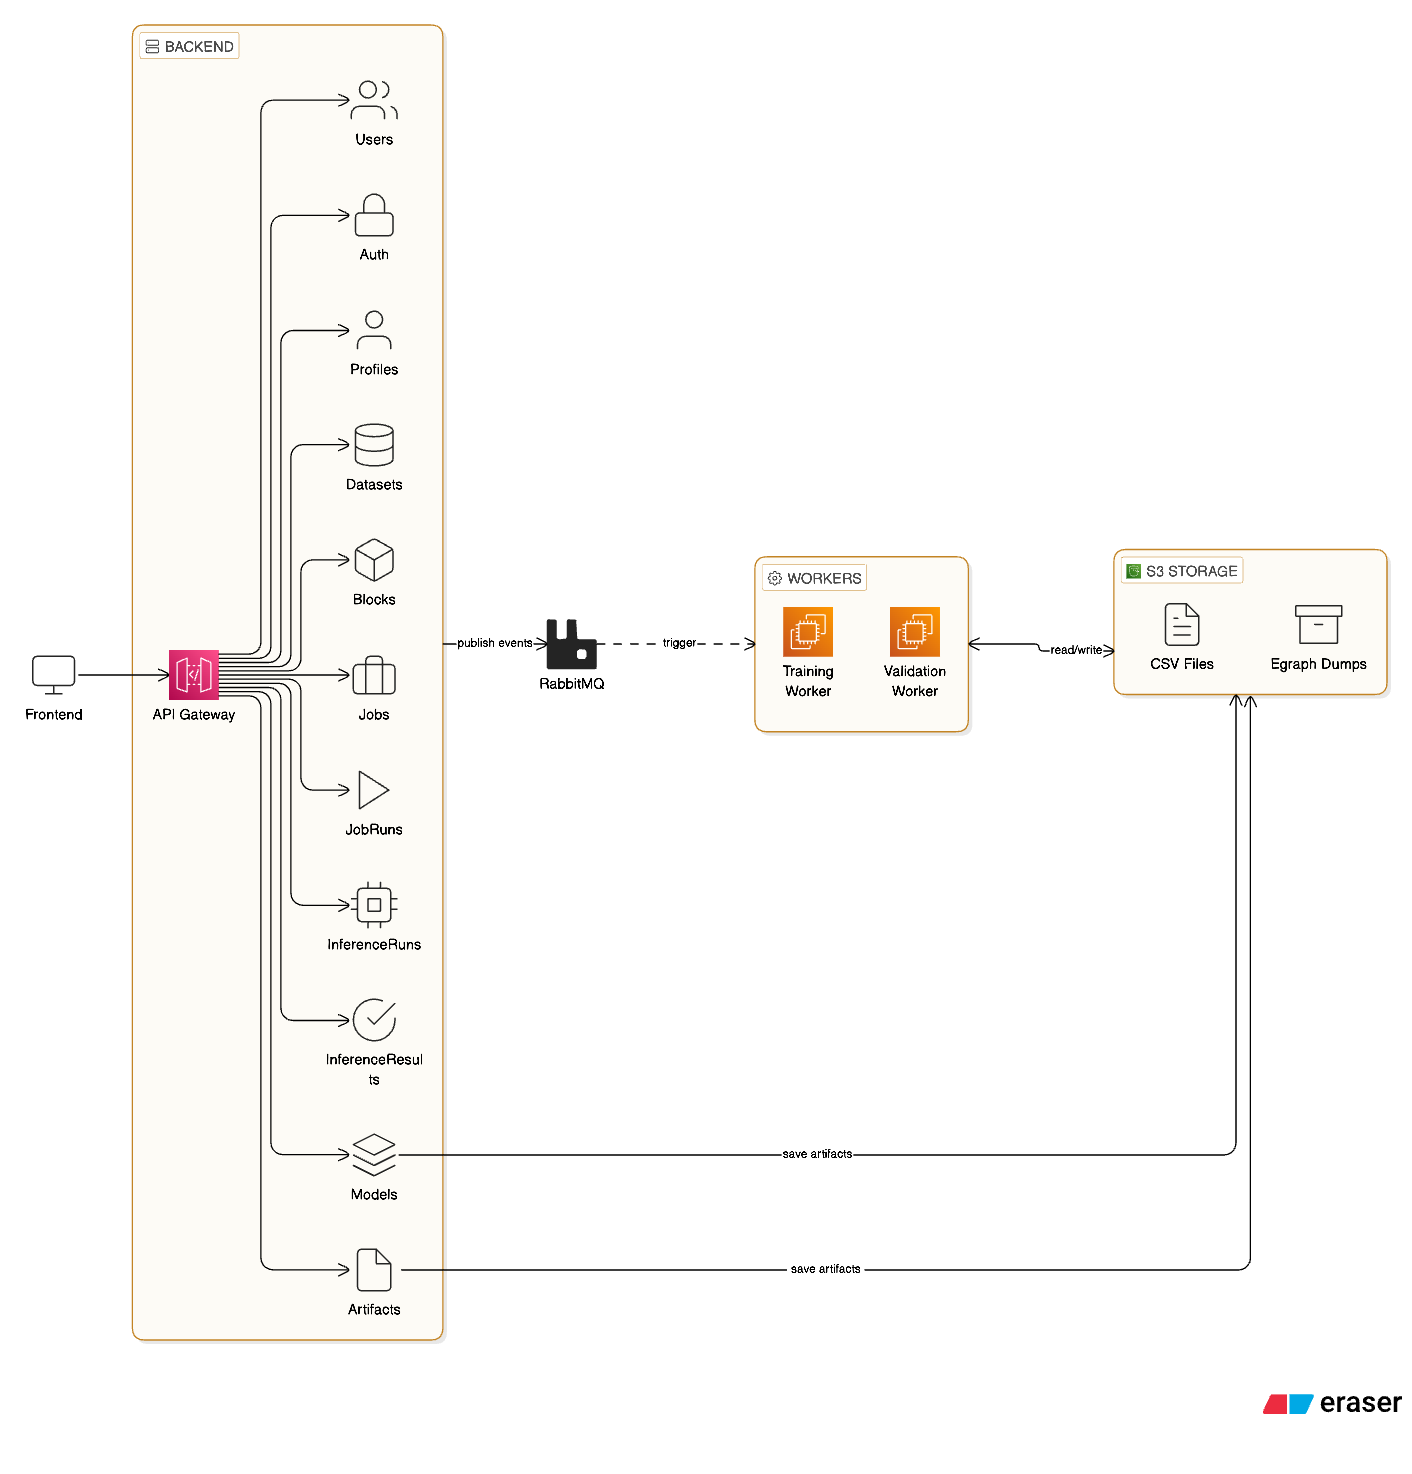
\includegraphics[width=0.8\textwidth]{images/high_level.png}
  \label{fig:high_level}
\end{figure}

O diagrama \ref{fig:high_level} apresenta a arquitetura de alto nível do projeto, dividida em quatro principais componentes:
\begin{enumerate}
    \item Front-end
    \item Back-end
    \item Workers
    \item Armazenamento
\end{enumerate}

\subsubsection{Front-End}
O front-end é responsável por mostrar ao usuário os dados vindos da API (\textit{Application Programming Interface}) e permitir a manipulacão desses dados. Por meio da interface, o usuário pode:
\begin{enumerate}
    \item Fazer upload de conjunto de dados
    \item Criar \textit{Profiles}, ou seja, espaços nos quais os conjuntos de dados podem ser importados para treinamento e manipulação de modelos
    \item Criar modelos de regressão simbólica para os conjuntos de dados de uma \textit{Profile}
    \item Gerenciar (atualziar e/ou excluir) conjuntos de dados e \textit{Profiles}
    \item Criar uma conta na plataforma
    \item Fazer login na conta criada
    \item Escrever scripts IQL para manipulação dos modelos criados
    \item Observar, por meio de elementos visuais como gráficos, propriedades dos modelos criados
\end{enumerate}

Toda comunicação com o back-end é feita de forma assíncrona, por meio de requisições HTTP ou \textit{Server Side Events (SSE)}, os quais permitem o back-end se comunicar diretamente com o front-end enviando dados via \textit{Streaming}.

\subsubsection{Back-End}
O back-end é resopnsável pelas regras de negócio da aplicação. Ele foi desenvolvido de forma modular, ou seja, cada módulo apresenta suas próprias regras de negócio e interfaces de comunicação próprias. É de responsabilidade do back-end também a comunicação com os demais serviços da plataforma, como os serviços de armazenamento (local ou S3, por exemplo), brokers de mensagens e \textit{workers}.

\begin{figure}
    \centering
    \caption{Diagrama de alto nível da arquitetura do back-end.}
    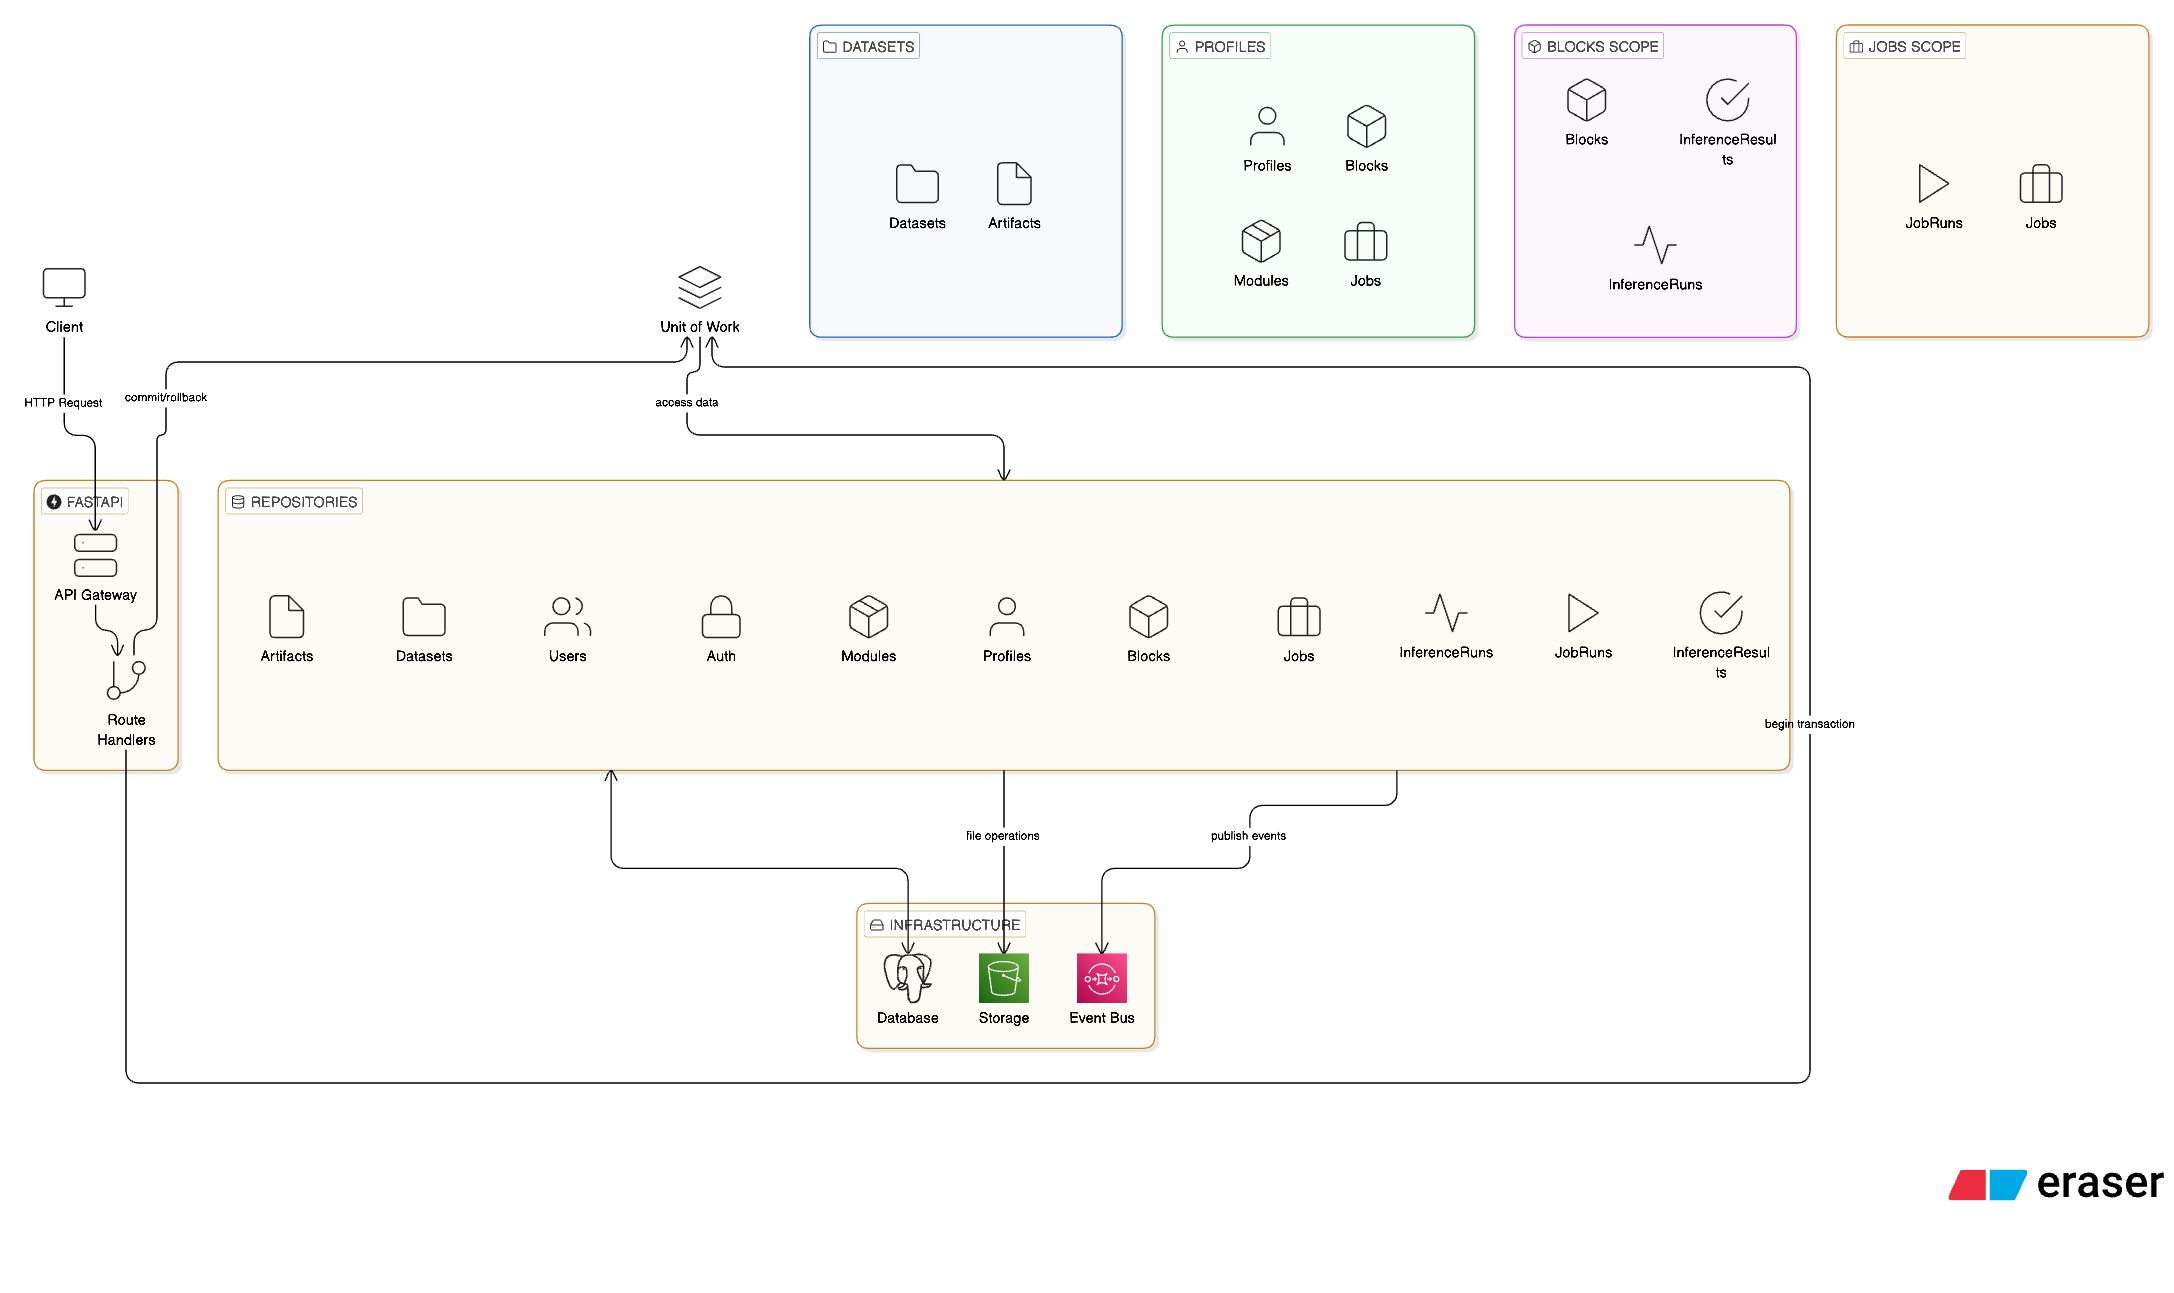
\includegraphics[width=0.8\textwidth]{images/backend.png}
    \label{fig:backend}
\end{figure}

O diagrama \ref{fig:backend} mostra o fluxo de uma requisição HTTP na aplicação, bem como a divisão de escopos para as entidades presentes. O principal padrão estrutural do back-end é o \textit{Unit of Work}, o qual possibilita retornar o estado da aplicação ao estado inicial caso um fluxo de mudanças encontre um erro. Esse padrão se utiliza de transações de banco de dados para garantir integridade do sistema (PROCURAR CITAÇÃO). As transações são controladas implicitamente pelo fluxo da aplicação Python, sendo automaticamente realizada a operação de \textit{commit} assim que o escopo da função responsável por determinada funcionalidade se encerra, ou sendo realizado o \textit{rollback} caso uma exceção seja levantada em código. Toda manipulação que necessita do banco de dados é realizada por meio de um repositório, o qual é uma classe que define operações base para cada entidade do sistema.

\subsubsection{Workers}
Os \textit{workers} são responsáveis por treinar os modelos de regressão utilizando a biblioteca \textit{eggp}~\cite{eggp}, e por validar os modelos criados, ou seja, calcular a fronteira de pareto do modelo e calcular os valores gerados por cada expressão de pareto. Assim como o \text{back-end}, as manipulações ao banco de dados são feitas via repositórios. O padrão \textit{Unit of Work} também é utilizado, mas, diferentemente do back-end, o controle das transações é feito de forma manual.

Cada \textit{worker} consume eventos específicos da fila de mensagens de forma assíncrona. Como cada \textit{worker} atualiza as informações pertinentes para seu domínio, não há comunicação no sentido dos \textit{workers} para o \textit{back-end}. No entanto, \textit{workers} podem se comunicar com a fila de mensagens, emitindo novos eventos para si mesmo ou outros \textit{workers}.

\subsubsection{Armazenamento}
O componente de armazenamento é responsável por armazenar os dados que não podem ser salvos no banco de dados, ou seja, artefatos necessários para o funcionamento da aplicação que não podem ser armazenados de forma tabular e relacional. Os principais elementos guardados nesse componente são:
\begin{enumerate}
    \item Arquivos CSV para os conjuntos de dados que cada usuário fez upload
    \item Arquivos para os e-graphs gerados pelo treinamento dos modelos
    \item Arquivos CSV gerados pelo treinamento dos modelos
\end{enumerate}

O componente de armazenamento apresenta dois modos de operação: modo local e modo remoto. No modo local, os arquivos são armazenados no sistema de arquivos do servidor que hospeda a aplicação. No modo remoto, os arquivos são armazenados em um S3, serviço da AWS para armazenar arquivos.

A interface de aramazenamento é definida de forma abstrata, por meio de protocolos, no pacote \textit{core}:
\begin{lstlisting}[language=Python, caption={Definição da interface de armazenamento}]
from typing import Protocol, BinaryIO
from .upload_result import UploadResult


class FileStorage(Protocol):
    async def upload(
        self,
        *,
        path: str,
        file: BinaryIO,
    ) -> UploadResult: ...

    async def download(
        self,
        *,
        path: str,
        destination: str,
    ) -> None: ...
\end{lstlisting}

Uma implementação para essa interface deve definir os métodos \textit{upload} e \textit{download}. Cada componente da aplicação que acessa o componente de armazenamento define sua própria implementação, permitindo que detalhes de implementção sejam escondidos do restante da aplicação que necessita utilizar esse componente. Esse padrão é chamado de \textit{Ports and Adapters} e permite a troca de implementações de serviços específicos dentro da aplicação desde que os métodos necessários sejam oferecidos por cada implementação. Abaixo, segue exemplo de implementação do serviço de armazenamento para o \textit{back-end}:
\begin{lstlisting}[language=Python, caption={Implementação da interface de armazenamento no back-end}]
import hashlib

from typing import BinaryIO
from pathlib import Path

from app.core.config import settings

from core.ports.storage.file_storage import FileStorage
from core.ports.storage.path import SpectrumPath
from core.ports.storage.upload_result import UploadResult


class LocalStorage(FileStorage):
    def __init__(self) -> None:
        self._base_path = Path(
            settings.FILE_STORAGE_SPECTRUM_DATA_PATH
        )

    async def upload(
        self,
        *,
        path: str,
        file: BinaryIO
    ) -> UploadResult:
        full_path = self._base_path / path
        full_path.parent.mkdir(parents=True, exist_ok=True)

        hasher = hashlib.sha256()
        size = 0

        file.seek(0)

        with open(full_path, 'wb') as f:
            while chunk := file.read(8192):
                f.write(chunk)
                hasher.update(chunk)
                size += len(chunk)

        spectrum_path = SpectrumPath(
            full_path=full_path, path=Path(path))
        checksum = hasher.hexdigest()

        return UploadResult(
            path=spectrum_path,
            size=size,
            checksum=checksum
        )

    async def download(
        self,
        *,
        path: str,
        destination: str
    ) -> None:
        source_path = self._base_path / path
        destination_path = Path(destination)

        if not source_path.exists():
            raise FileNotFoundError(
                f"File not found at path: {source_path}")

        destination_path.parent.mkdir(
            parents=True, exist_ok=True)
        destination_path.write_bytes(source_path.read_bytes())
\end{lstlisting}
